% Choose one to switch betweeen slides and handout
\documentclass[]{beamer}
%\documentclass[handout]{beamer}

% Video Meta Data
\title{Smart Contracts \& Blockchain Applications}
\subtitle{Blockchain Overview}
\author{Prof. Dr. Fabian Schär}
\institute{University of Basel}

% Config File
% Packages
\usepackage[utf8]{inputenc}
\usepackage{hyperref}
\usepackage{gitinfo2}
\usepackage{tikz}
 \usetikzlibrary{calc}
\usepackage{amsmath}
\usepackage{mathtools}
\usepackage{bibentry}
\usepackage{xcolor}
\usepackage{colortbl} % Add colour to LaTeX tables
\usepackage{caption}
\usepackage[export]{adjustbox}
\usepackage{pgfplots} \pgfplotsset{compat = 1.17}
\usepackage{makecell}
\usepackage{fancybox}
\usepackage{ragged2e}
\usepackage{fontawesome}
\usepackage{seqsplit}
\usepackage{tabularx}
\usepackage{tcolorbox}
\usepackage{booktabs} % use instead  \hline in tables

% Color Options
\definecolor{highlight}{rgb}{0.65,0.84,0.82}
\definecolor{focus}{rgb}{0.72, 0, 0}
\definecolor{lightred}{rgb}{0.8,0.5,0.5}
\definecolor{midgray}{RGB}{190,195,200}

 %UniBas Main Colors
\definecolor{mint}{RGB}{165,215,210}
\definecolor{anthracite}{RGB}{45,55,60}
\definecolor{red}{RGB}{210,5,55}

 %UniBas Color Palette (for graphics)
\definecolor{strongmint}{RGB}{30,165,165}
\definecolor{darkmint}{RGB}{0,110,110}
\definecolor{softanthracite}{RGB}{140,145,150}
\definecolor{brightanthracite}{RGB}{190,195,200}
\definecolor{softred}{RGB}{235,130,155}

%Custom Colors
\definecolor{lightergray}{RGB}{230, 230, 230}



% Beamer Template Options
\beamertemplatenavigationsymbolsempty
\setbeamertemplate{footline}[frame number]
\setbeamercolor{structure}{fg=black}
\setbeamercolor{footline}{fg=black}
\setbeamercolor{title}{fg=black}
\setbeamercolor{frametitle}{fg=black}
\setbeamercolor{item}{fg=black}
\setbeamercolor{}{fg=black}
\setbeamercolor{bibliography item}{fg=black}
\setbeamercolor*{bibliography entry title}{fg=black}
\setbeamercolor{alerted text}{fg=focus}
\setbeamertemplate{items}[square]
\setbeamertemplate{enumerate items}[default]
\captionsetup[figure]{labelfont={color=black},font={color=black}}
\captionsetup[table]{labelfont={color=black},font={color=black}}

\setbeamertemplate{bibliography item}{\insertbiblabel}

%tcolor boxes
\newtcolorbox{samplecode}[2][]{
  colback=mint, colframe=darkmint, coltitle=white,
  fontupper = \ttfamily\scriptsize, fonttitle= \bfseries\scriptsize,
  boxrule = 0mm, arc = 0mm,
  boxsep = 1.3mm, left = 0mm, right = 0mm, top = 0.5mm, bottom = 0mm, middle=0mm,
  #1,title=#2}
  
\newtcolorbox{keytakeaway}[2][]{
  colback=softred, colframe=red, coltitle=white,
  fontupper = \scriptsize, fonttitle= \bfseries\scriptsize,
  boxrule = 0mm, arc = 0mm,
  boxsep = 1.3mm, left = 0mm, right = 0mm, top = 0.5mm, bottom = 0mm, middle=0mm,
  #1,title=#2}

\newtcolorbox{exercise}[2][]{
  colback=brightanthracite, colframe=anthracite, coltitle=white,
  fontupper = \scriptsize, fonttitle= \bfseries\scriptsize,
  boxrule = 0mm, arc = 0mm,
  boxsep = 1.3mm, left = 0mm, right = 0mm, top = 0.5mm, bottom = 0mm, middle=0mm,
  #1,title=#2}



% Link Icon Command 
\newcommand{\link}{%
    \tikz[x=1.2ex, y=1.2ex, baseline=-0.05ex]{%
        \begin{scope}[x=1ex, y=1ex]
            \clip (-0.1,-0.1)
                --++ (-0, 1.2)
                --++ (0.6, 0)
                --++ (0, -0.6)
                --++ (0.6, 0)
                --++ (0, -1);
            \path[draw,
                line width = 0.5,
                rounded corners=0.5]
                (0,0) rectangle (1,1);
        \end{scope}
        \path[draw, line width = 0.5] (0.5, 0.5)
            -- (1, 1);
        \path[draw, line width = 0.5] (0.6, 1)
            -- (1, 1) -- (1, 0.6);
        }
    }

% Other commands
\newcommand\tab[1][0.5cm]{\hspace*{#1}} % for code boxes


% Read Git Data from Github Actions Workflow
% Defaults to gitinfo2 for local builds
\IfFileExists{gitInfo.txt}
	{\input{gitInfo.txt}}
	{
		\newcommand{\gitRelease}{(Local Release)}
		\newcommand{\gitSHA}{\gitHash}
		\newcommand{\gitDate}{\gitAuthorIsoDate}
	}

% Custom Titlepage
\defbeamertemplate*{title page}{customized}[1][]
{
  \vspace{-0cm}\hfill\includegraphics[width=2.5cm]{../config/logo_cif}
  \includegraphics[width=1.9cm]{../config/seal_wwz}
  \\ \vspace{2em}
  \usebeamerfont{title}\textbf{\inserttitle}\par
  \usebeamerfont{title}\usebeamercolor[fg]{title}\insertsubtitle\par  \vspace{1.5em}
  \small\usebeamerfont{author}\insertauthor\par
  \usebeamerfont{author}\insertinstitute\par \vspace{2em}
  \usebeamercolor[fg]{titlegraphic}\inserttitlegraphic
    \tiny \noindent \texttt{Release Ver.: \gitRelease}\\ 
    \texttt{Version Hash: \gitSHA}\\
    \texttt{Version Date: \gitDate}\\ \vspace{1em}
    
    
    \iffalse
  \link \href{https://github.com/cifunibas/Bitcoin-Blockchain-Cryptoassets/blob/main/slides/intro.pdf}
  {Get most recent version}\\
  \link \href{https://github.com/cifunibas/Bitcoin-Blockchain-Cryptoassets/blob/main/slides/intro.pdf}
  {Watch video lecture}\\ 
  
  \fi
  
  \vspace{1em}
  License: \texttt{Creative Commons Attribution-NonCommercial-ShareAlike 4.0 International}\\\vspace{2em}
  \includegraphics[width = 1.2cm]{../config/license}
}


% tikzlibraries
\usetikzlibrary{decorations.pathreplacing}
\usetikzlibrary{decorations.markings}
\usetikzlibrary{positioning}
\usetikzlibrary{calc}
\captionsetup{font=footnotesize}

%%%%%%%%%%%%%%%%%%%%%%%%%%%%%%%%%%%%%%%%%%%%%%
%%%%%%%%%%%%%%%%%%%%%%%%%%%%%%%%%%%%%%%%%%%%%%
\begin{document}

\thispagestyle{empty}
\begin{frame}[noframenumbering]
	\titlepage
\end{frame}

%%%
\begin{frame}{Blockchain Origin}

\centering
\includegraphics[width = 5cm, frame]{../assets/images/nakamoto_cover}
		
\textbf{Bitcoin: A Peer-to-Peer Electronic Cash System} \\ 
Satoshi Nakamoto \\
\link \href{https://bitcoin.org/bitcoin.pdf}{Online version}

\end{frame}
%%%

%%%
\begin{frame}{Payment Systems: Today's Challenge}

Physical Cash: Presence in the same place at the same time
\begin{figure}[h]
	\center
		\input{../assets/figures/cash_payment.tex}
\end{figure}

\vspace{1.5 em}

\uncover<2->{Digital Cash: Proof of ownership
\begin{figure}[h]
	\center
		\input{../assets/figures/ecash_payment.tex}
\end{figure}}
	
\end{frame}
%%%	


%%%
\begin{frame}{Today's Solution: Intermediaries Keeping Money Registries}

\begin{figure}[h]
	\center
		\input{../assets/figures/registry_payment.tex}
\end{figure}

\uncover<2->{\vspace{1 em}

\textbf{Registry Types}\\
\vspace{1 em}
\textbf{Implicit:} Verbal agreements, limited to small groups.\\
\textbf{Explicit:} Records in written or digital databases.}
	
\end{frame}
%%%	


%%%
\begin{frame}{Implicit Registry Example: The Stone Money of Yap}
	\center
	\includegraphics[width=8cm]{../assets/images/yap_stones}\\
	\footnotesize{Picture source: Eric Guinther}
\end{frame}
%%%


%%%
\begin{frame}{Implicit Registry Example: The Stone Money of Yap}

\begin{figure}[h]
	\center
		\input{../assets/figures/yap_system.tex}
\end{figure}
	
\end{frame}
%%%

%%%
\begin{frame}{Scaling the Yap Network}
	\begin{figure}
			\input{../assets/figures/yap_network.tex}
	\end{figure}
	\vspace{1em}
	\uncover<4->{
		\textbf{Large network size results in three problems:}
		\begin{itemize}
			\item<5-> Transaction capacity
			\item<6-> Transaction legitimacy
			\item<7-> Transaction consensus
		\end{itemize}
	}
	\vspace{1em}
	
\uncover<8->{
	\begin{alertblock}{Key idea}
		Blockchains as decentralized data structures that are maintained by its participants in the absence of a centralized third party. 	
	\end{alertblock}
}
\end{frame}
%%%


%%%
\begin{frame}{Transaction Capacity}
\textbf{Goal:} Ensure that each participant can reliably \color{focus}initiate a transaction \color{black} without having to fear censorship. \\
\uncover<2->{
	\begin{figure}[h!]
		\center
		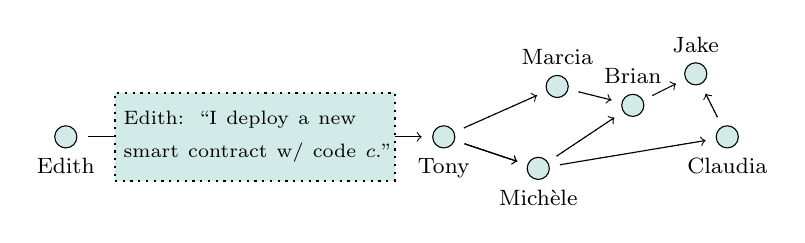
\begin{tikzpicture}[domain=-8:8, scale=0.8]

% transaction
\uncover<3->{
	\coordinate (c1) at (0,0);
	\coordinate (c2) at (6,0);
	\filldraw[draw=black,fill=highlight!50] (c1) circle (5pt) node[below=0.15cm,color=black]{\footnotesize{Edith}};
	\draw[shorten >=0.28cm,shorten <=0.28cm,->] (c1) to[] (c2);
}

% network
\uncover<2->{
\coordinate (c3) at (7.8,0.8);
\coordinate (c4) at (7.5,-0.5);
\coordinate (c5) at (9,0.5);
\coordinate (c6) at (10,1);
\coordinate (c7) at (10.5,0);
\filldraw[draw=black,fill=highlight!50] (c2) circle (5pt) node[below=0.15cm,color=black]{\footnotesize{Tony}};
\filldraw[draw=black,fill=highlight!50] (c3) circle (5pt) node[above=0.15cm,color=black]{\footnotesize{Marcia}};
\filldraw[draw=black,fill=highlight!50] (c4) circle (5pt) node[below=0.15cm,color=black]{\footnotesize{Michèle}};
\filldraw[draw=black,fill=highlight!50] (c5) circle (5pt) node[above=0.15cm,color=black]{\footnotesize{Brian}};
\filldraw[draw=black,fill=highlight!50] (c6) circle (5pt) node[above=0.15cm,color=black]{\footnotesize{Jake}};
\filldraw[draw=black,fill=highlight!50] (c7) circle (5pt) node[below=0.15cm,color=black]{\footnotesize{Claudia}};
}

\uncover<3->{
\draw[shorten >=0.28cm,shorten <=0.28cm,->] (c2) to[] (c3);
\draw[shorten >=0.28cm,shorten <=0.28cm,->] (c2) to[] (c4);
\draw[shorten >=0.28cm,shorten <=0.28cm,->] (c2) to[] (c4);
\draw[shorten >=0.28cm,shorten <=0.28cm,->] (c3) to[] (c5);
\draw[shorten >=0.28cm,shorten <=0.28cm,->] (c4) to[] (c5);
\draw[shorten >=0.28cm,shorten <=0.28cm,->] (c4) to[] (c7);
\draw[shorten >=0.28cm,shorten <=0.28cm,->] (c5) to[] (c6);
\draw[shorten >=0.28cm,shorten <=0.28cm,->] (c7) to[] (c6);
}

\uncover<2>{
\draw[shorten >=0.28cm,shorten <=0.28cm, dotted] (c2) to[] (c3);
\draw[shorten >=0.28cm,shorten <=0.28cm, dotted] (c2) to[] (c4);
\draw[shorten >=0.28cm,shorten <=0.28cm, dotted] (c2) to[] (c4);
\draw[shorten >=0.28cm,shorten <=0.28cm, dotted] (c3) to[] (c5);
\draw[shorten >=0.28cm,shorten <=0.28cm, dotted] (c4) to[] (c5);
\draw[shorten >=0.28cm,shorten <=0.28cm, dotted] (c4) to[] (c7);
\draw[shorten >=0.28cm,shorten <=0.28cm, dotted] (c5) to[] (c6);
\draw[shorten >=0.28cm,shorten <=0.28cm, dotted] (c7) to[] (c6);
}

% value transaction
\uncover<3>{
\filldraw[fill=highlight!50,dotted,thick] (0.78,-0.7) -- (5.22,-0.7) -- (5.22,0.7) -- (0.78,0.7) -- (0.78,-0.7) node[midway, right=-0.02cm,text width=4.25cm]{\scriptsize{Edith: ``I transfer one \\ Ether to Daniel.''}};
}

% smart contract interaction
\uncover<4>{
\filldraw[fill=highlight!50,dotted,thick] (0.78,-0.7) -- (5.22,-0.7) -- (5.22,0.7) -- (0.78,0.7) -- (0.78,-0.7) node[midway, right=-0.02cm,text width=4.25cm]{\scriptsize{Edith: ``Execute function \\ $f$ of \texttt{0x...} with data $d$.''}};
}

% smart contract deployment
\uncover<5>{
\filldraw[fill=highlight!50,dotted,thick] (0.78,-0.7) -- (5.22,-0.7) -- (5.22,0.7) -- (0.78,0.7) -- (0.78,-0.7) node[midway, right=-0.02cm,text width=4.25cm]{\scriptsize{Edith: ``I deploy a new \\ smart contract w/ code $c$.''}};
}


\end{tikzpicture}

	\end{figure}\vspace{1em}
}
\uncover<2->{
	Peer-to-Peer Network:
        \begin{itemize}
		\item<1-> Permissionless
		\item<1-> Censorship-resistant
		\item<1-> No special privileges
		\end{itemize}
		}
\end{frame}
%%%


%%%
\begin{frame}{Transaction Legitimacy}
\textbf{Goal:} Ensure transaction \color{focus}authenticity \color{black}and \color{focus} integrity\color{black}, i.e., ensure that the transaction was initiated by its owner of the funds and has not been changed.
\uncover<2->{
		\center
		\input{../assets/figures/transaction-legit.tex}
		}
\uncover<3->{
		\vspace{1em}
		\input{../assets/figures/transaction-manipulation.tex}
	}
\end{frame}
%%%


%%%
\begin{frame}{Transaction Consensus}
\textbf{Goal: }Deciding which (legitimate) transactions are valid. \\
\vspace{1em}
\uncover<2->{
Potential Problem: Assume both transactions have valid signatures, but spend the same Bitcoin units. What now? \\
\begin{figure}[h!]
	\center
	\input{../assets/figures/double-spend.tex}
\end{figure}
}
\end{frame}
%%%

%%%
\begin{frame}{Recommended Reading}
\begin{columns}
	\begin{column}{0.3\textwidth}
	\center
	\includegraphics[width=\textwidth , frame]{../assets/images/short-introduction-cryptocurrencies.png}
	\end{column}
	\begin{column}{0.7\textwidth}
	\textbf{A Short Introduction to the World of Cryptocurrencies} \\
	Aleksander Berentsen and Fabian Schär \\
	\link \href{https://files.stlouisfed.org/files/htdocs/publications/review/2018/01/10/a-short-introduction-to-the-world-of-cryptocurrencies.pdf}{Online PDF}
	\end{column}
\end{columns}
\end{frame}
%%%


\end{document}